\documentclass{jarticle}
\usepackage{mathtools, multicol}
\usepackage{color}
\usepackage{url}
\usepackage{comment}
\usepackage{here}
\usepackage{txfonts}
\usepackage{listings, jlisting}
\usepackage{latexsym}
\usepackage{subfigure}

\renewcommand{\lstlistingname}{リスト}

\lstdefinestyle{customplain}{
  belowcaptionskip=1\baselineskip,
  breaklines=true,
  frame=tRBl,
  xleftmargin=\parindent,
  language=,
  showstringspaces=false,
  numbers=left,
  basicstyle=\footnotesize\ttfamily,
  keywordstyle=\bfseries\color{black},
  commentstyle=\itshape\color{black},
  identifierstyle=\color{black},
  stringstyle=\color{black},
}

% 余白の設定
\usepackage[top=20truemm, bottom=16truemm, left=10truemm, right=10truemm]{geometry}

% 図の挿入
\usepackage[dvipdfm]{graphicx}

% より複雑な数学記号
\usepackage{amsmath,amssymb}

% 図の通し番号
\usepackage{subfigure}

\newcommand{\todayd}{%
\the\year.{\ifnum \month < 10 0\the\month \else \the\month \fi}.%
{\ifnum \day < 10 0\the\day \else \the\day \fi}}


\makeatletter

\def\@thesis{人工知能}
\def\id#1{\def\@id{#1}}
\def\department#1{\def\@department{#1}}

\def\@maketitle{
	\begin{center}
		{\huge \@thesis \par} %大きなタイトルが記載される部分
		\vspace{10mm}
		{\LARGE\bf \@title \par} % タイトル部分
		\vspace{20mm}
		{\Large 提出締切: 2013.12.18\par} % 提出年月日部分
		\vspace{5mm}
		{\Large 提出日:  \@date \par} % 提出年月日部分
		\vspace{20mm}
		{\Large \@department \par} % 所属部分
		\vspace{10mm}

		{\Large\@id } % 学籍番号部分
		{\Large \@author} % 氏名 
	\end{center}
\par\vskip 1.5em
}

\makeatother

\title{第5回講義課題 課題番号15}
\date{\todayd}
\department{工学部電子情報工学科}
\id{03-123006}
\author{岩成達哉}


\begin{document}

\begin{titlepage}
	\setlength{\topmargin}{1.1in}
	\vspace{100mm}
	\maketitle
\end{titlepage}


\section{概要}
立体$4$目並べに対して,UCTアルゴリズムを適用し,試行回数によって,勝敗がどのように変化するかを調べた.また,Negamaxに$\alpha \beta$カットを用いたプログラムと対戦させ,勝敗や探索の効率(展開されたノード数,実行時間など)を比較した.




% -----
\section{立体$4$目並べ}
題材とした立体$4$目並べについて説明する.


\subsection{道具}
立体$4$目並べは,$4 \times 4$の盤面が$4$つ重なった図\ref{fig:board}のような盤面上でゲームが進行する.実際には図\ref{fig:real_board}のように$16$本の棒が立っており,図\ref{fig:put_stone}のように石を置いていく.石は,図\ref{fig:put_stone}のように黒と白の$2$種類があり,それぞれ$32$個ずつある.

\begin{figure}[H]
\centering
	\subfigure[立体$$4目並べの盤面]{
		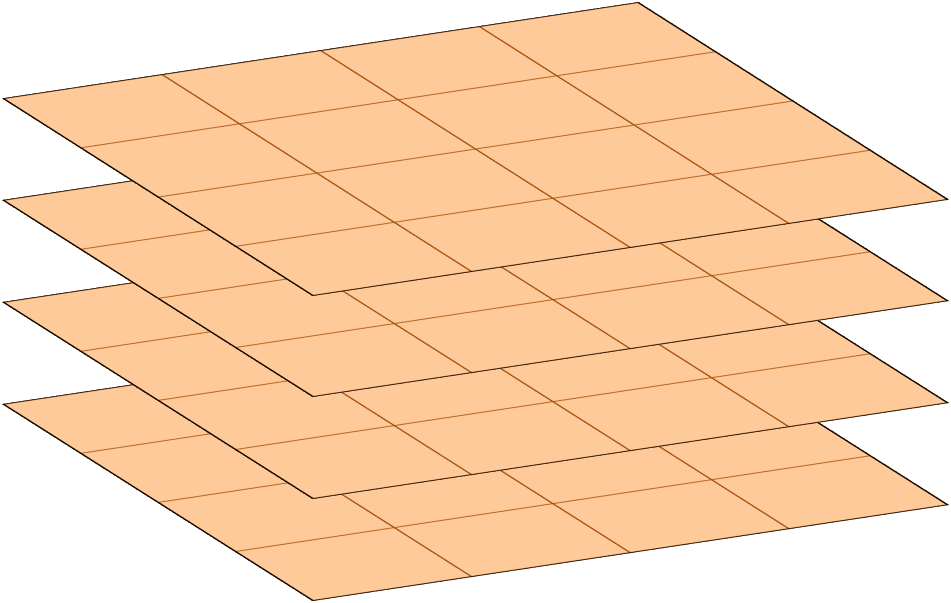
\includegraphics[width=60mm]{image/board.png}
		\label{fig:board}}
	\subfigure[実際の立体$4$目並べの構造]{
		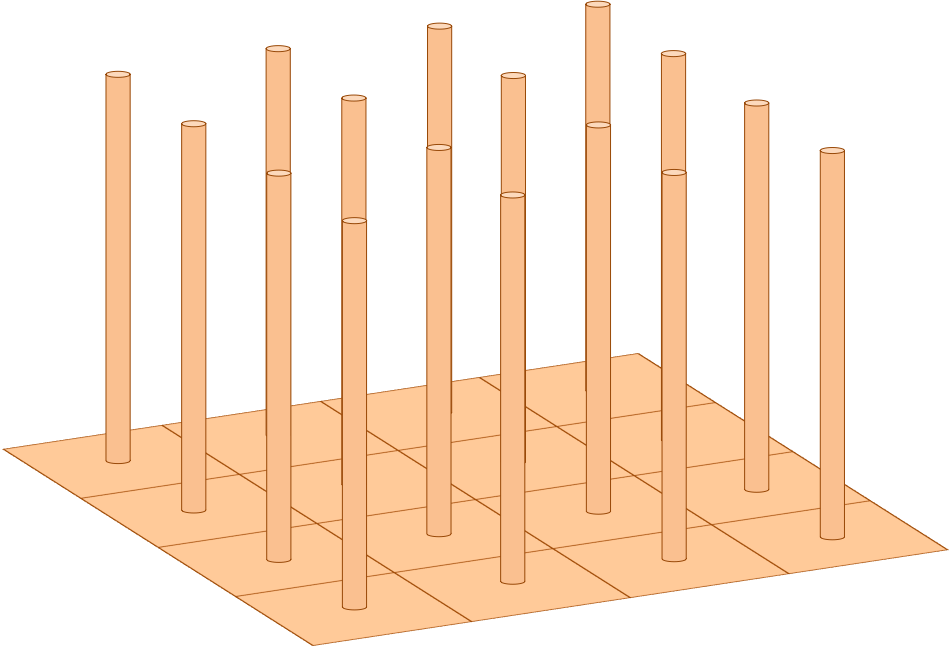
\includegraphics[width=60mm]{image/real_board.png}
		\label{fig:real_board}}
	\subfigure[石の設置]{
		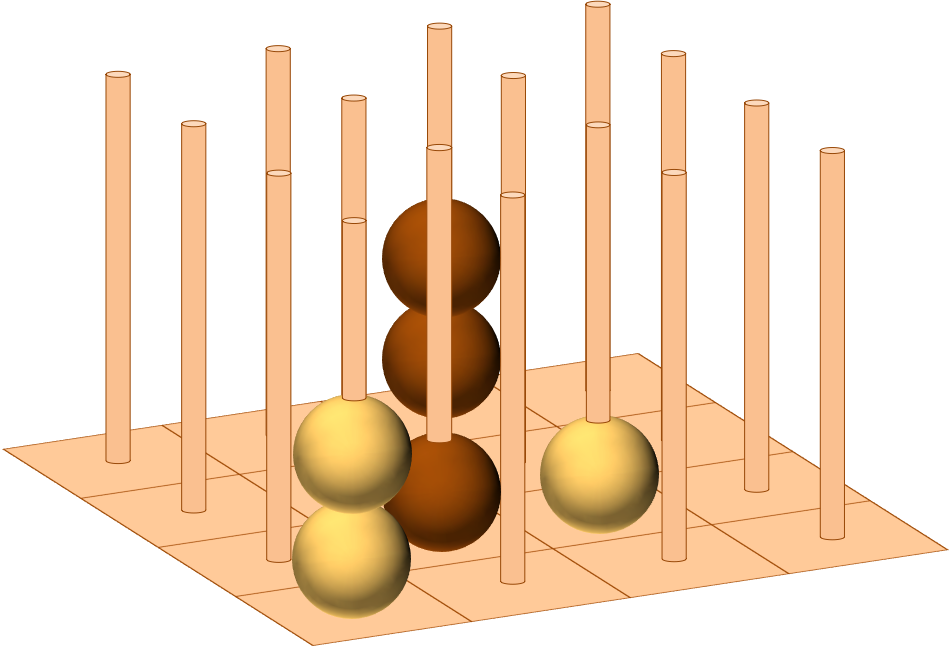
\includegraphics[width=60mm]{image/put_stone.png}
		\label{fig:put_stone}}
	\caption{ゲームの盤面}
	\label{fig:game_board}
\end{figure}




\subsection{ゲームの流れ}
立体$4$目並べは$2$人で行う対戦ゲームである.$2$人のプレイヤーが交互に自分の色の石を置いていき,先に勝利条件を満たした者が勝ちとなる.石は,図\ref{fig:game_board}で示した盤面に置いていくが,石を浮かせることは出来ず,一番下から順に積んでいく.



\subsection{勝利条件}
立体$4$目並べは,$3$次元的に縦,横,斜めに同じ色の石を$4$つ揃えた者の勝利である.例えば,図\ref{fig:win_example}のような並びで黒が勝利となる.図\ref{fig:board}でも示したように$4$つの平面によって成り立つため,図\ref{fig:plane_win}の条件がそれぞれの面で成立し得る.また,図\ref{fig:win}や図\ref{fig:diagonal_win}のような場合も$3$次元的に縦,横,斜めに配置できているため,黒の勝利といえる.
\begin{figure}[H]
\centering
	\subfigure[平面での勝利]{
		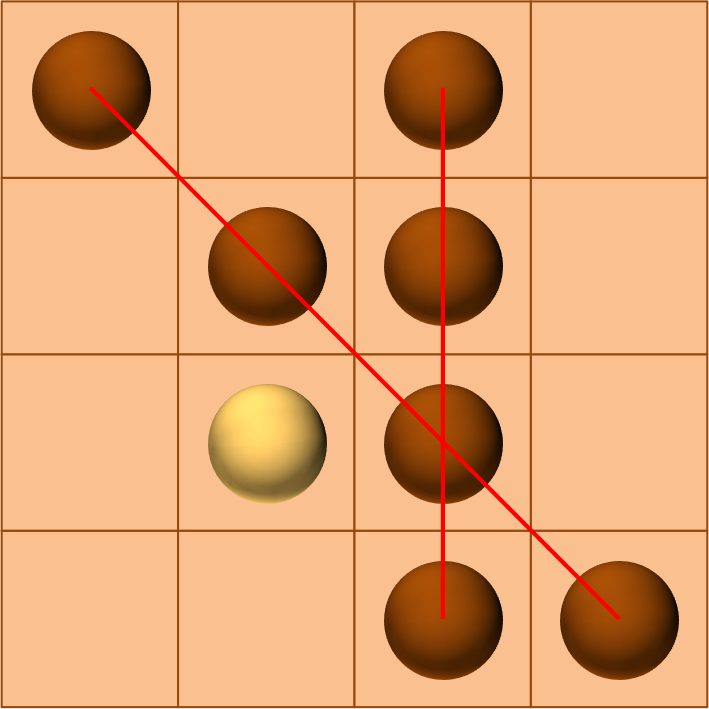
\includegraphics[width=50mm]{image/plane_win.png}
		\label{fig:plane_win}}
	\subfigure[横の面での勝利]{
		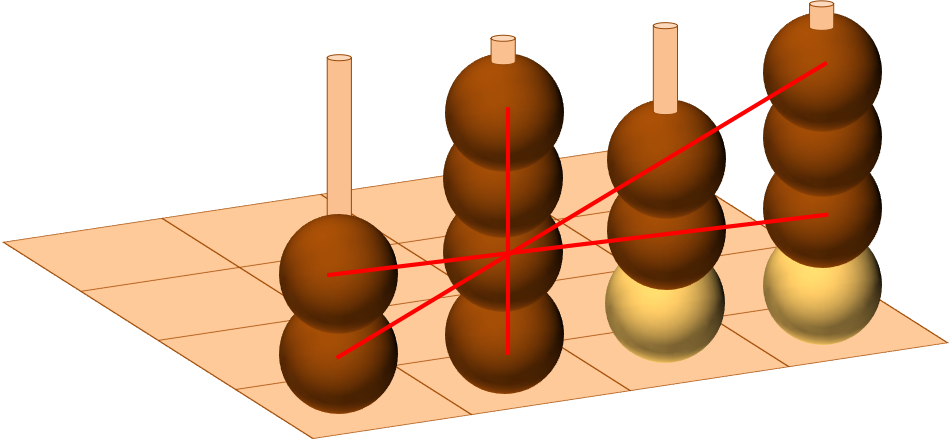
\includegraphics[width=65mm]{image/win.png}
		\label{fig:win}}
	\subfigure[対角線での勝利]{
		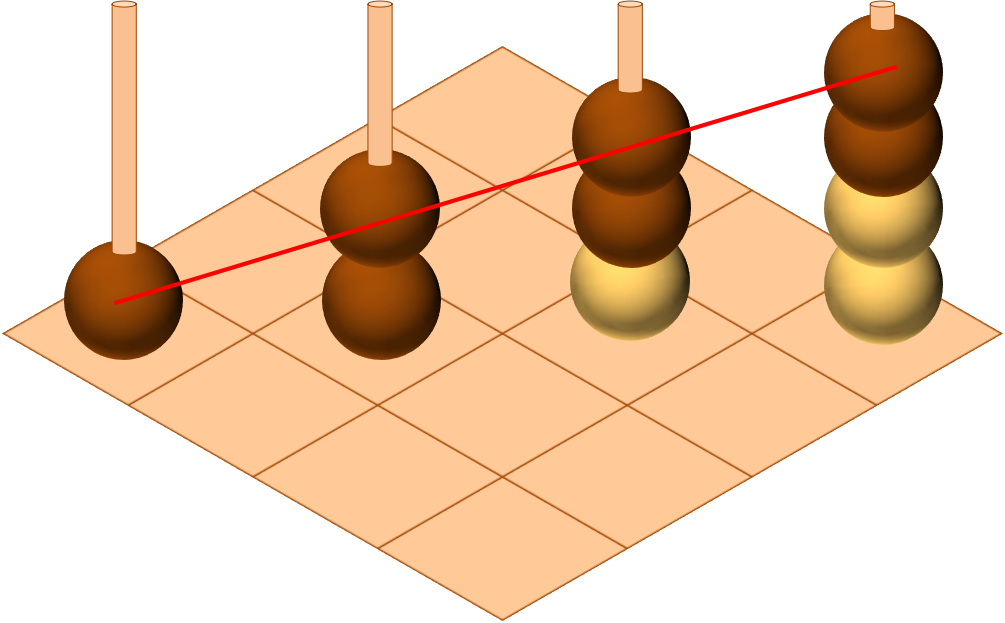
\includegraphics[width=65mm]{image/diagonal_win.png}
		\label{fig:diagonal_win}}
	\caption{黒が勝利する例}
	\label{fig:win_example}
\end{figure}





% ---
\section{実装したプログラムの仕様}

\subsection{実行環境}
プログラムの動作環境を表\ref{fig:spec}に示した.動作環境がMac OS,Linuxとなっているのは,時間を図るためにシステムコールを用いるgettimeofday関数を使用しているからである.提出したファイルでは,コメントアウトしているため,Windowsでも実行は可能である.
\begin{table}[htdp]
	\caption{プログラムの動作環境}
	\begin{center}
		\begin{tabular}{|c|c|c|c|} \hline 
			言語 & 開発環境 & コンパイラ & 動作環境 \\ \hline \hline 
			C & Mac OS X (Mavericks) & gcc & Mac OS , Linux(Windows) \\ \hline 
		\end{tabular}
	\end{center}
	\label{fig:spec}
\end{table}


\subsection{実行方法}
プログラムのコンパイルは,添付したMakefileによって行える.コマンドラインで,AI\_123006\_15のフォルダに移動し,下記のコマンドを打ち,Enterキーを押す.
\lstset{style=customplain}
\begin{lstlisting}[caption={make},label=code:make]
> make
\end{lstlisting}
正常に動作すれば,mainというファイルが生成されるため,
\begin{lstlisting}[caption={実行},label=code:execute]
> ./main
\end{lstlisting}
と入力し,Enterキーを押すことで実行できる.

本アプリケーションは,コマンドラインからの引数で対戦方法を指定できる.これをリスト\ref{code:option}に示した.
\begin{lstlisting}[caption={実行},label=code:option]
> ./main [先手:0, 後手:その他(デフォルト:0)] [UCTの総プレイアウト回数(デフォルト:10000)]
\end{lstlisting}




\subsection{使用方法}
アプリケーションの使用方法を以下に示した.

先手の場合を考える.アプリケーションを実行すると,リスト\ref{code:first}のような表示がプロンプトに現れる.
\lstset{style=customplain}
\lstinputlisting[caption={手の打ち方},label=code:first]{source/first.txt}

これは,上から$4$段目,$3$段目...の$16$マスを表している.プレイヤーは,guideにしたがって,$0$〜$15$の数値を入力し,Enterキーを押す.すると,指定した位置に石が置かれ,その様子をリスト\ref{code:second}に示した.\lstset{style=customplain}
\lstinputlisting[caption={置いた結果},label=code:second]{source/second.txt}

次に,PCがUCTを用いて,手を打つ.これをリスト\ref{code:third}に示した.
\lstset{style=customplain}
\lstinputlisting[caption={相手の手番},label=code:third]{source/third.txt}

次に,リスト\ref{code:first}のようなguideが表示され,プレイヤーが打つ.以上を繰り返し,どちらかが勝利するか引き分けになればその旨が表示される.

% ---
\section{アルゴリズムの概要}

\subsection{勝利条件の判定}
立体$4$目並べでは,勝利パターンが数多く存在し,それを判定する必要がある.

まず,$4 \times 4$の面においての勝利判定を用意する.これは,置かれた位置を中心に,その前後左右,斜めに$4$つ同じ色の石が並んでいるか判定すればよい.

次に,置いてある位置を中心とした,最大で$4$つの面を作る.この様子を図\ref{fig:planes}に示した.

図\ref{fig:3planes}は,置かれた位置がどこであっても生成する判定すべき面である.置かれた位置に対して$3$つの方向に面を作り,それぞれの面に対して,前述の勝利判定を行えばよい.

一方,置かれた位置が図\ref{fig:board}で表した$4$つの面のいずれかの対角線上に置かれた場合は,図\ref{fig:diagonal_win}のようなパターンで勝利する可能性があるため,この面についても前述の勝利判定を行う.

\begin{figure}[H]
\centering
	\subfigure[基本となる3つの面]{
		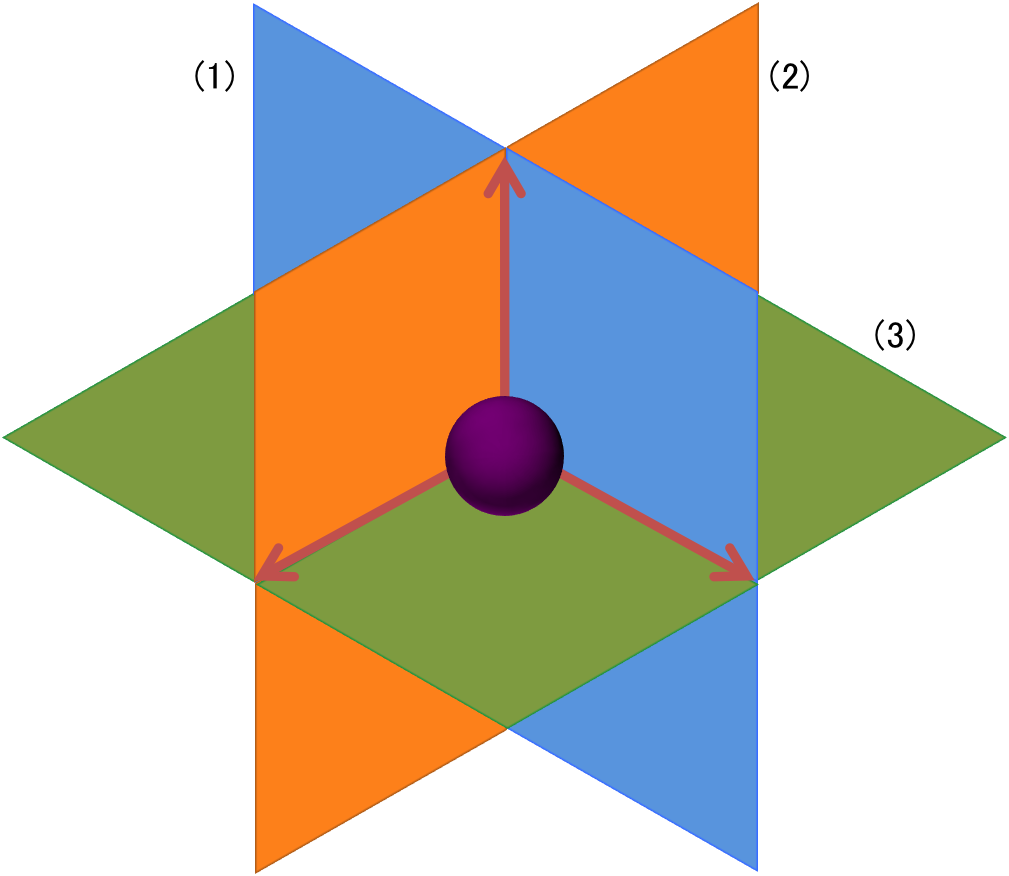
\includegraphics[width=70mm]{image/3planes.png}
		\label{fig:3planes}}
	\subfigure[斜めの面]{
		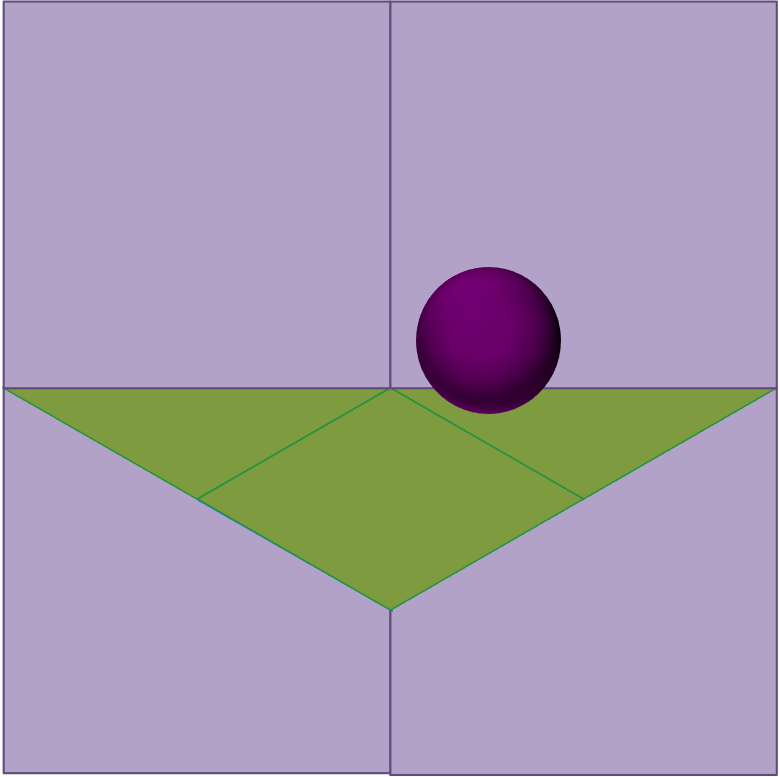
\includegraphics[width=50mm]{image/diagonal_plane.png}
		\label{fig:diagonal_plane}}
	\caption{判定を行う面}
	\label{fig:planes}
\end{figure}



\subsection{合法手の作成}
UCTやNegamax法では,合法手の作成が必須である.立体$4$目並べでは,一番上の面(下から$4$番目の面)の,すでに石が置かれている位置には石が置けないという以外,白と黒の石を置く位置に制限はない.よって,一番上の面の$16$個を確認すれば良い.


\subsection{UCTの概要\cite{ref:book}}
UCT(UCb applied to Trees)は,モンテカルロ木探索にUCB値を用いて,探索するノードの優先度をつける手法である.UCB値は,以下の式で与えられる.
\begin{eqnarray}
\label{eq:ucb}
	&&UCB = (\pm) X_i + C \sqrt{\frac{\ln n}{n_i}} \\
	ただし,&&符号は自分の手番の手なら+,相手の手番の手なら-,\nonumber \\
	&&X_iはそのノードの勝率,Cは定数, nは総プレイアウト回数,n_iはそのノードのプレイアウト回数 \nonumber
\end{eqnarray}
この値が最も大きくなる手をランダムにゲームオーバーまで探索する.また,あるノードのプレイアウト回数が一定値を超えた際は,そのノードをさらに展開(次の手も子として持つ)し,プレイアウトを行う.その結果は,親に向かって伝播させる.

これによって,有力な手は次々に展開されていく.また,展開した手が,相手の手番の手である場合は,UCB値の勝率の符号を判定させて,相手が相手にとって有利な手を打つことを想定するようにした.

参考文献\cite{ref:book}を基に,これを実装した.

\subsection{Negamax $+ \alpha \beta$カットの概要\cite{ref:book}\cite{ref:negamax}}
Negamax法は,MinMax法を改良した方式である.

MinMax法は,「自分は自分の評価値が最大となる手を指し,相手は自分の評価値が最小となる手を指す」という仮定でアルゴリズムを組んでおり,自分と相手の手を指すのは別の関数となる.一方,NegaMax法は「自分も相手も自身の評価値が最大となる手を指す」ということを仮定し,相手の評価値は符号を反転して評価に加える.これによって,同じ関数を用いることができ,実装が容易となる.

このNegamax法に,$\alpha \beta$枝刈りを導入したプログラムを作成した.Negamaxの評価関数は,$4 \times 4 \times 4$の評価値を経験から入力しておき,それを用いて計算する単純な方式を用いた.リーチの数を求めて評価に加える方法もあったが,後述のように十分強いAIとなったため,この実装は行わなかった.



\subsection{工夫した点}
UCTでは,勝率を計算するために,勝ったときのみそれをカウントするため,式(\ref{eq:ucb})の勝率$X_i$はもちろん正である.しかし,今回扱った立体$4$目並べでは,負ける組み合わせ(同時に勝つ組み合わせ)が膨大であり,「負ける」という情報を大きく扱うべきと考える.

よって,今回実装したUCTアルゴリズムでは,負けた時は勝った回数を$-1$することで,$X_i$が負の値を取りうるように変更した.つまり,Negamaxの考え方をUCTに導入したといえる.



% ---
\section{実験方法}
実験は,学科PC(Ubuntu 12.04 [Intel Core i7 @2.40GHz,8コア,メモリ16GB])によって行った.

\subsection{Cの決定}
\label{sec:seek_c}
UCTで用いる式(\ref{eq:ucb})では,定数$C$を用いている.この値は実験によって決める値となっているため,最も勝率が高くなるような$C$を求めるために実験を行った.実験方法は以下のとおりである.UCTを先手とした.
\begin{enumerate}
	\item Negamax法のプログラム(探索の深さ$5$)のプログラムを対戦相手とした
	\item UCTの総プレイアウト回数を$1000$,展開の閾値を$50$として,$C$を変化させて500回戦わせ勝率を求めた
	\item 総プレイアウト回数が$2000$,$5000$,$10000$,$20000$,$50000$でも$C$を変化させて勝率を求めた
\end{enumerate}

展開の閾値を$50$としたのはあらかじめ実験を行って求めた結果からである.


\subsection{UCT同士の対戦}
UCTアルゴリズム同士の対戦でプレイアウト回数を変化させた時の勝率の変化を調べた.実験方法は以下のとおりである.勝率は先手のものを求めた.
\begin{enumerate}
	\item UCTの総プレイアウト回数を$1000$,展開の閾値を$50$,$C=0.6$を敵とした
	\item UCTの総プレイアウト回数を変化させたものと500回戦わせて勝率を求めた
	\item 敵の総プレイアウト回数を$2000$,$5000$,$10000$,$20000$,$50000$と変化させて同様の操作を行った
\end{enumerate}




\subsection{UCTとNegamaxの対戦と探索効率}
UCTとNegamaxの対戦を行い,その勝率を求めた.このとき,$C$は\ref{sec:seek_c}節の実験から$C=0.6$を採用した.実験方法は以下のとおりである.UCTを先手とした.

\begin{enumerate}
	\item Negamax法(探索の深さ$1$)のプログラムを対戦相手とした
	\item UCTの総プレイアウト回数を$1000$,展開の閾値を$50$として$C$を変化させて500回戦わせ勝率を求めた
	\item 総プレイアウト回数が$2000$,$5000$,$10000$,$20000$,$50000$でも$C$を変化させて勝率を求めた
	\item Negamax法の探索を$2,3,..,6$と増やし,同様の実験を行った.
\end{enumerate}

また,探索の効率をUCTとNegamaxで比較を行った.比較は,展開されたノード数と実行時間を調査することで行った.
UCTの探索効率を測る実験の方法は以下のとおりである.

\begin{enumerate}
	\item $1$手目での展開されたノード数(探索の深さ)と実行時間を比較した
	\item 試行回数$1000$のUCTを用いて,1手目を打つことを$100$回繰り返し,その合計時間を求めた
	\item 手を繰り返す際に,一番深く進んだ深さの$100$回の平均を求めた
	\item 同様の内容を試行回数を変化させて行った
\end{enumerate}

Negamaxの探索効率を測る実験の方法は以下のとおりである.
\begin{enumerate}
	\item 深さ$1$のNegamaxを用いて,1手目を打つことを$100$回繰り返し,その合計時間を求めた
	\item 同様の内容を深さを変化させて行った
\end{enumerate}



% ---
\section{結果}
\subsection{Cの決定}
Cを求める実験の結果を図\ref{fig:seek_C}に示した.結果から,$C=0.5$〜$0.7$の時に勝率が大きくなっていることがわかった.

\begin{figure}[H]
	\centering
	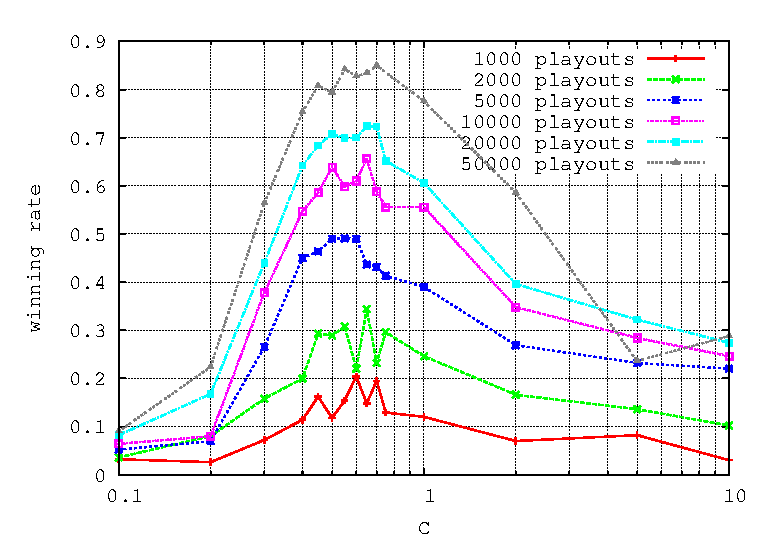
\includegraphics[width=130mm]{image/seek_C.eps}
	\caption{最適なCの調査\label{fig:seek_C}}
\end{figure}




\subsection{UCT同士の対戦}
UCT同士の対戦結果を図\ref{fig:vs_uct}に示した.$x$軸は先手のプレイアウト回数であり,後手のプレイアウト回数を固定して実験を行い,先手の勝率を$y$軸にとって示した.この結果から,試行回数を増やすと勝率が向上していることがわかった.

\begin{figure}[H]
	\centering
	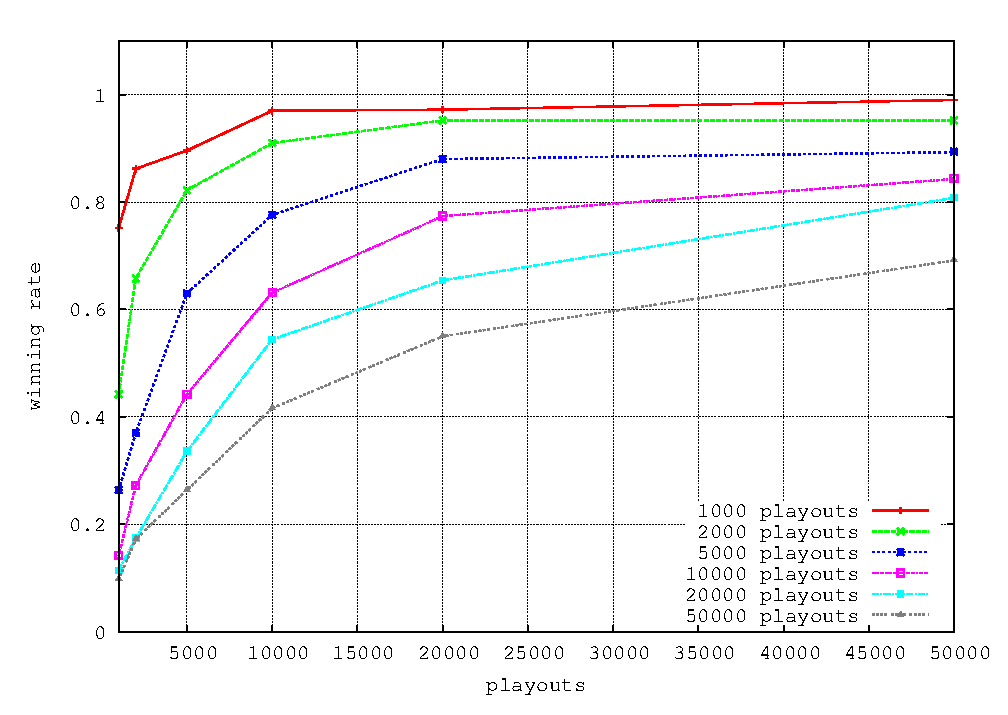
\includegraphics[width=130mm]{image/vs_uct.eps}
	\caption{UCT同士の対戦\label{fig:vs_uct}}
\end{figure}


\subsection{UCTとNegamaxの対戦と探索効率}
UCTとNegamaxの対戦結果を図\ref{fig:vs_negamax}に示した.この結果から,深さ$1$のNegamax法に対しては,負けることがなく,深さ$6$のNegamax法に対しても試行回数が$10000$を超えれば勝率が$50 \% $以上となることがわかった.

\begin{figure}[H]
	\centering
	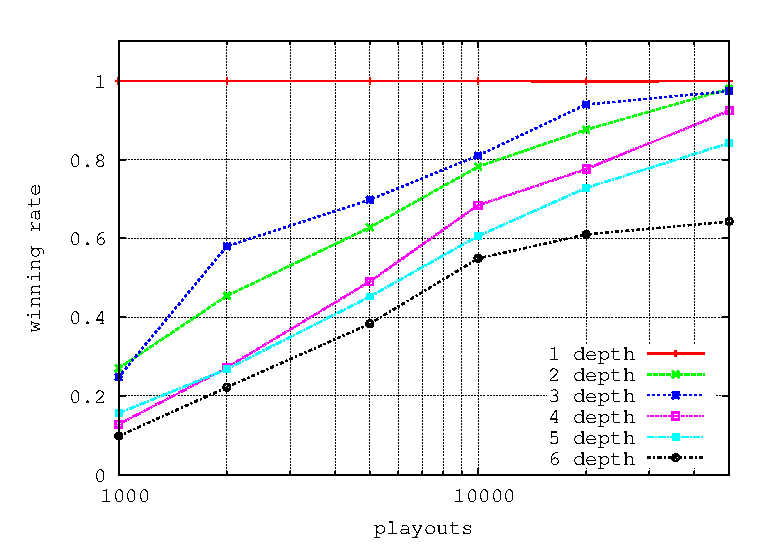
\includegraphics[width=130mm]{image/vs_negamax.eps}
	\caption{Negamaxとの対戦\label{fig:vs_negamax}}
\end{figure}

また,探索効率の実験結果を図\ref{fig:search}に示した.これによって,UCTは試行回数にともなって線形に探索時間が変化し,探索の深さは徐々に大きくなっていくことがわかった.$400000$回の試行で深さの平均は$8$となった.一方,Negamaxは探索の深さを変化させると,指数関数的に増加することがわかった.これらは,アルゴリズム通りの結果である.

\begin{figure}[H]
\centering
	\subfigure[UCTの探索効率]{
		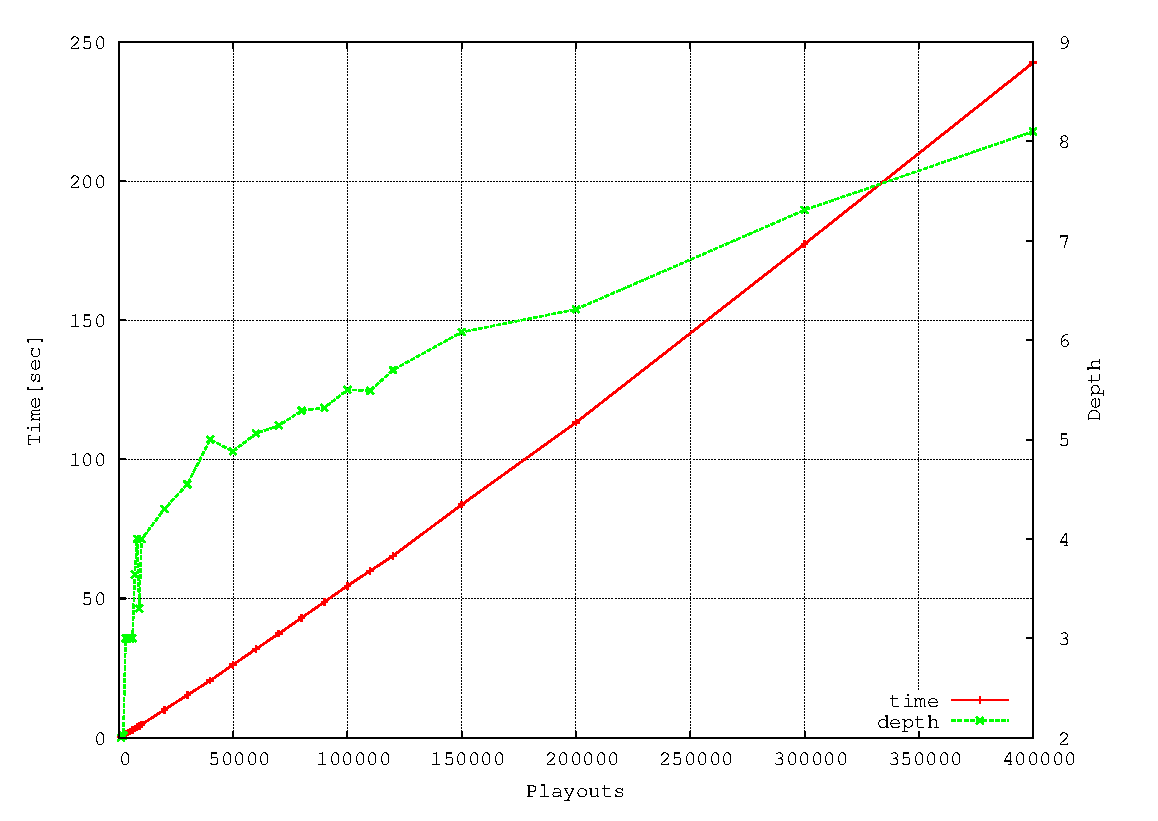
\includegraphics[width=150mm]{image/search_uct.eps}
		\label{fig:search_uct}}
	\subfigure[Negamaxの探索効率]{
		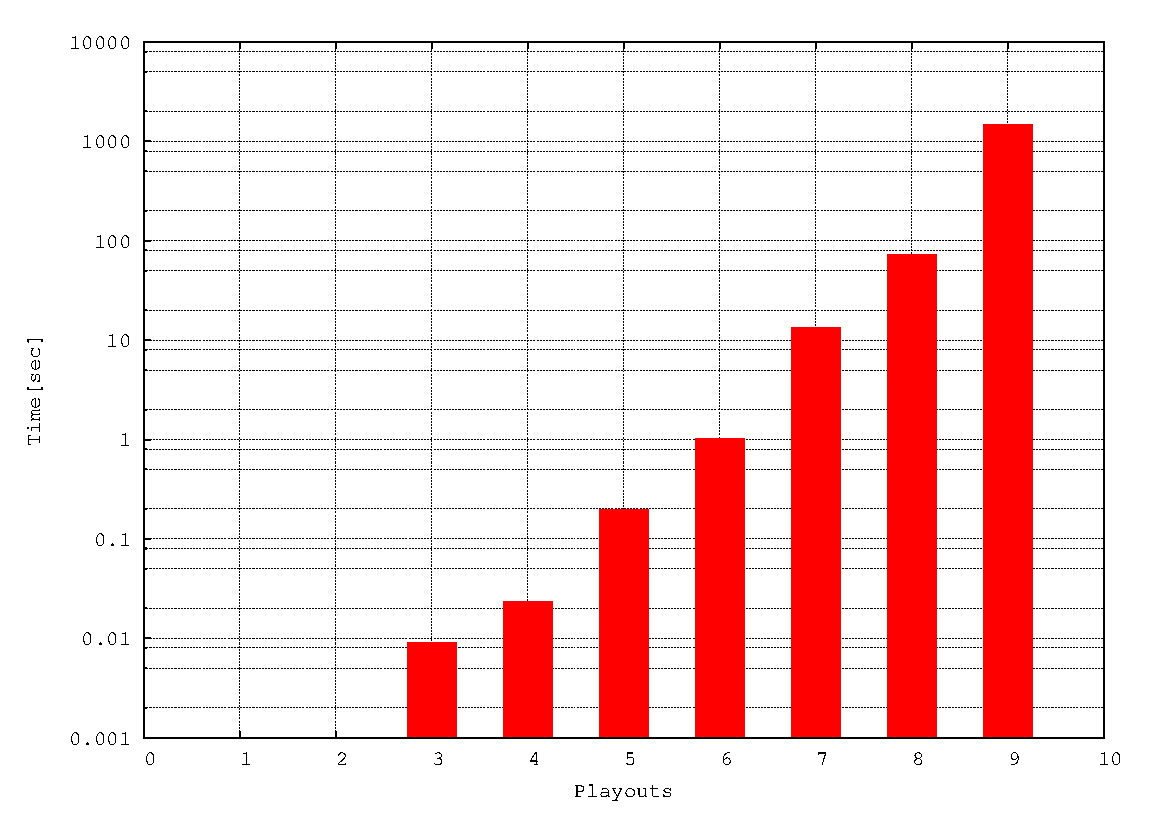
\includegraphics[width=150mm]{image/search_negamax.eps}
		\label{fig:search_negamax}}
	\caption{探索効率}
	\label{fig:search}
\end{figure}




% ---
\section{考察}
\subsection{$C$の決定}
$C$を求めた結果,$C$が$0.5$よりも小さい時や,$0.7$よりも大きい時は勝率が低くなった.そもそも$C$は,UCB値の第$2$項の影響をどの程度考慮するかを決める値である.UCB値の第$1$項は勝率の高さ,第$2$項は探索した回数が少ないことをそれぞれ優先する.

したがって,$C$が小さければ勝率のみを重視して探索を行うため,偶発的に勝利,あるいは敗北した手に対して,探索が効率よく行われない.また,逆に$C$が大きすぎれば,勝率よりも探索の回数が少ないものが重視されるため,全ての手をまんべんなく試行するようになる.つまり幅優先に近い動作をすると考えられる.これによって,探索の深さが浅くなり,良い結果が得られない.

今回は,およそ$0.5$〜$0.7$の間で勝率が良くなったため,その平均の$0.6$を使用して他の実験を行った.



\subsection{UCT同士の対戦}
UCT同士の対戦では,試行回数を増やしていくと,勝率が上昇していく様子がわかった.したがって,プログラムが正しく動作しているとかんがえられる.

試行回数が同じときを見てみると,プレイアウト回数が$1000$回のときに$0.75$である以外は,いずれも$0.6$程度となっているとわかる.つまり,このゲームは先手のほうが勝率が高くなるゲームであると考えられ,実力が同程度であれば$0.6$程度の勝率になると推察される.


\subsection{UCTとNegamaxの対戦と探索効率}
UCTとNegamaxの対戦では,試行回数を増やすとNegamaxに対して勝率が上昇した.前述のとおり先手が有利であると考えると,深さ$6$のNegamaxは,プレイアウト回数が$2〜50000$回のUCTの強さに相当すると推察できる.

一方で,探索の効率の結果を見ると,深さ$6$のNegamaxは$1$秒で$100$回探索が行えるが,プレイアウト回数が$50000$回のUCTでは,$26$秒が$100$回探索にかかっているため,UCTのほうが効率が悪いといえる.

一方で,UCTの展開の深さの平均は,$50000$回のときに$5$となっている.よって,平均すると$5$手先まで見ることで深さ$6$のNegamaxと同等の強さを持つこととなり,この点では効率が良いといえる.これは,有望な手をUCB値によって正しく定められているからであると推察される.

また,Negamaxは試行にかかる時間が指数的に上昇する.Negamaxは,深さを$7$とすると,深さ$6$のときのおよそ$10$倍の時間がかかる.一方で,UCTでは,試行回数$50000$回から$150000$回,あるいは$200000$回から$270000$回などのようにおよそ$100000$回で深さが一つ増えるが,試行にかかる時間は線形であるため,強くするにはUCTのほうが有利であることが推察される.


%---
\section{結論}
UCTアルゴリズムを用いて,立体$4$目並べのAIを実装し,Negamax$+\alpha \beta$アルゴリズムと対戦させた.その結果,UCTの効率の良さと強くしやすさが分かる結果となった.立体$4$目並べは,比較的評価関数が作りやすいため,Negamax法でも十分な強さとなったが,評価関数が作成しにくいゲームでは,UCTアルゴリズムのほうがより有利になると考えられる.


\begin{thebibliography}{n}
\bibitem{ref:book}
伊庭 斉志 :『人工知能と人工生命の基礎』,オーム社 (2013.5.24)

\bibitem{ref:negamax}
『MinMax法とNegaMax法』(last accessed 2013.12.13),\url{http://www.es-cube.net/es-cube/reversi/sample/html/2_4.html}

\end{thebibliography}

\section*{付録}
\subsection*{ソースリスト}
ソースのリストを以下に示した.

\begin{itemize}
	\item Makefile \\
		makeをするためのファイル
	\item board.c / board.h \\
		盤面についての処理をまとめたもの.盤面の表示や勝利判定,盤面のコピー,Undoなどが定義されている.
	\item uct.c / uct.h \\
		UCTアルゴリズムを実装したもの.
	\item negamax.c / negamax.h \\
		Negamax法 $ + \alpha \beta$カットを実装したもの.
	\item main.c \\
		ゲームの進行をするもの.ユーザからの入力などを受け付ける.
\end{itemize}

\end{document}



\lstset{style=customplain}
\lstinputlisting[caption={A,B,Cの記述},label=code:description]{source/description_abc.txt}











